\documentclass[conference,final]{IEEEtran}

\usepackage{latex8}
\usepackage{times}

\usepackage[utf8]{inputenc}
\usepackage{url}
\usepackage{float}
\usepackage{times}    
\usepackage{multirow}    
\usepackage{listings}   
\usepackage{times}     
\usepackage{paralist}    
\usepackage{wrapfig}    
\usepackage[small,it]{caption}
\usepackage{multirow}
\usepackage{ifpdf}
\usepackage{srcltx}


\usepackage{listings}
\usepackage{keyval}  
\usepackage{color}
\definecolor{listinggray}{gray}{0.95}
\definecolor{darkgray}{gray}{0.7}
\definecolor{commentgreen}{rgb}{0, 0.4, 0}
\definecolor{darkblue}{rgb}{0, 0, 0.4}
\definecolor{middleblue}{rgb}{0, 0, 0.7}
\definecolor{darkred}{rgb}{0.4, 0, 0}
\definecolor{brown}{rgb}{0.5, 0.5, 0}

\lstdefinestyle{myListing}{
  frame=single,   
  backgroundcolor=\color{listinggray},  
  %float=t,
  language=C,       
  basicstyle=\ttfamily \footnotesize,
  breakautoindent=true,
  breaklines=true
  tabsize=2,
  captionpos=b,  
  aboveskip=0em,
  belowskip=-2em,
  %numbers=left, 
  %numberstyle=\tiny
}      

\lstdefinestyle{myPythonListing}{
  frame=single,   
  backgroundcolor=\color{listinggray},  
  %float=t,
  language=Python,       
  basicstyle=\ttfamily \footnotesize,
  breakautoindent=true,
  breaklines=true
  tabsize=2,
  captionpos=b,  
  %numbers=left, 
  %numberstyle=\tiny
}

\newcommand{\up}{\vspace*{-1em}}
\newcommand{\upp}{\vspace*{-0.5em}}
\newcommand{\numrep}{8 }
\newcommand{\samplenum}{4 }
\newcommand{\tmax}{$T_{max}$ }
\newcommand{\tc}{$T_{C}$ }
\newcommand{\tcnsp}{$T_{C}$}
\newcommand{\bj}{BigJob}

% This is now the recommended way for checking for PDFLaTeX:
\usepackage{ifpdf}

%\newif\ifpdf
%\ifx\pdfoutput\undefined
%\pdffalse % we are not running PDFLaTeX
%\else
%\pdfoutput=1 % we are running PDFLaTeX
%\pdftrue
%\fi

\ifpdf
\usepackage[pdftex]{graphicx}
\else
\usepackage{graphicx}
\fi
\title{A Pilot-Job-based, Data-affinity-aware MapReduce Implementation}
\author{  }


\begin{document}

\ifpdf
\DeclareGraphicsExtensions{.pdf, .jpg, .tif}
\else
\DeclareGraphicsExtensions{.eps, .jpg}
\fi

\maketitle


\section{Introduction}

Many problems at the forefront of science, engineering, medicine, and the social 
sciences, are increasingly data-intensive. MapReduce is a well-known programming 
model for expressing distributed computations on large amounts of data.

In this paper we present an infrastructure-independent SAGA-based framework for 
MapReduce. In contrast to our earlier work~\cite{Sehgal2011590} we utilize the 
SAGA Python-binding to lower the barrier of entry for scientist. Also, we  
utilize the SAGA-based Pilot-Job and Pilot-Data abstractions to efficiently 
manage data and compute tasks.

Managing data affinities both within MapReduce runs, e.\,g.\ during the shuffle 
phase, and between multiple MapReduce runs, e.\,g.\ in an iterative MapReduce 
scenario, is important to achieve an acceptable performance.


In this paper we demonstrate:
\begin{itemize}
	\item How to efficiently utilize SAGA-based P* abstractions for implementing 
	MapReduce.
	\item MR framework is interoperable with different infrastructures (cloud 
	and grid)
	\item We perform different experiments on various heterogeneous 
	infrastructures (FutureGrid, AWS, TG)
\end{itemize}



What is different in our MR implementation?
When to go distribute? When not?



\section{Related Work}

\begin{itemize}
	\item Jon Weissman paper
	\item Google Paper, GAE MapReduce
	\item Microsoft Dryad
	\item Hadoop
	\item Iterative MapReduce
\end{itemize}


\section{MapReduce Application Characteristics}

MapReduce applications can be classified as follows~\cite{weissman2011,ramakrishnan2011}:
\begin{itemize}
    \item Data-intensive applications show a significant higher I/O rate in proportion to the used CPU cycles. Such applications can be well described using Amdahl's number~\cite{gray2000}. Another characteristic particular useful for MapReduce is the data aggregation and flow through the system:
        \begin{itemize}
            \item High aggregation: The output of the MapReduce job is significant smaller than the input.
            \item Zero Aggregation: The MapReduce output is the same as the 
            input.
            \item Ballooning data: The output is larger than the input.
        \end{itemize}
    \item Compute-intensive applications are dominated by CPU cycles. Input 
    files are usually small and thus, I/O is not an issue.
    \item Memory-intensive require that a significant amount of data is load
    into the memory, which is usually the case for computer- and data-intensive 
    applications.
\end{itemize}
Further characteristics of data-intensive applications refer to~\cite{jha2011}.



\section{Pilot*-Abstractions for MapReduce}

\subsection{Pilot-Job}

\subsection{Pilot-Data}
Figure~\ref{fig:extension_figures_pilot-data-mapreduce} shows the utilization of 
Pilot Data within the MapReduce framework.
\begin{figure*}[htbp]
	\centering
	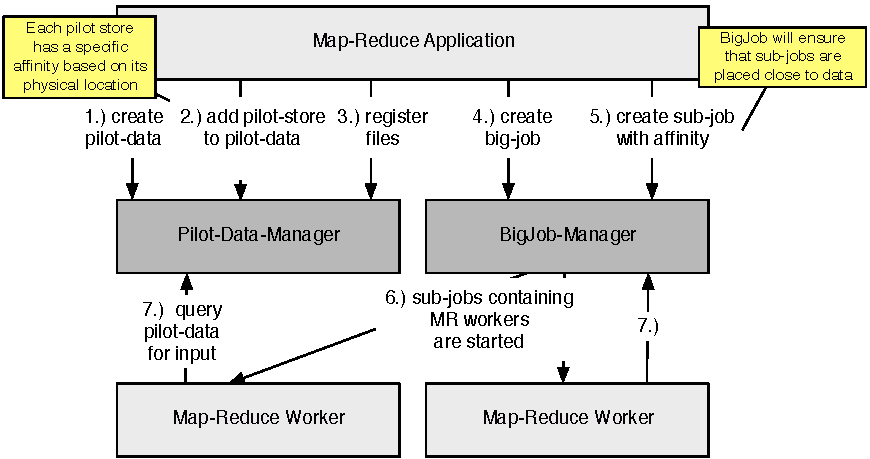
\includegraphics[width=\textwidth]{../extension/figures/pilot-data-mapreduce.pdf}
	\caption{Pilot-Data and MapReduce}
	\label{fig:extension_figures_pilot-data-mapreduce}
\end{figure*}


\section{SAGA MapReduce Architecture}


\section{Implementation and Experiments}
Scenarios:
\begin{itemize}
	\item 1 BJ 16 core 1 machine
	\item 2 BJ 8 cores - 1 machines
	\item 2 BJ 8 cores - 2 machines
\end{itemize}



Other parameters:
\begin{itemize}
	\item placement of data
	\item cloud
\end{itemize}

\bibliographystyle{plain}
\bibliography{../extension/pilotjob.bib,../../../Compiled_bibentries/saga.bib}
\end{document}
